% !TEX root = ../Ausarbeitung.tex
\section{Funktionalität von Container}
\label{sec:Funktionalität von Container}

Container setzen direkt auf dem Kernel eines Linux-Betriebssystems auf. Um auf den Kernel durchgreifen zu können, verwenden Container standard Linux-Techniken wie Cgroups und Namespaces oder selbst entwickelte Schnittstellen. Dadurch wird das Betriebssystem innerhalb des Containers, ohne vollständige Virtualisierung emuliert.
\begin{figure}[H]
	\begin{center}
		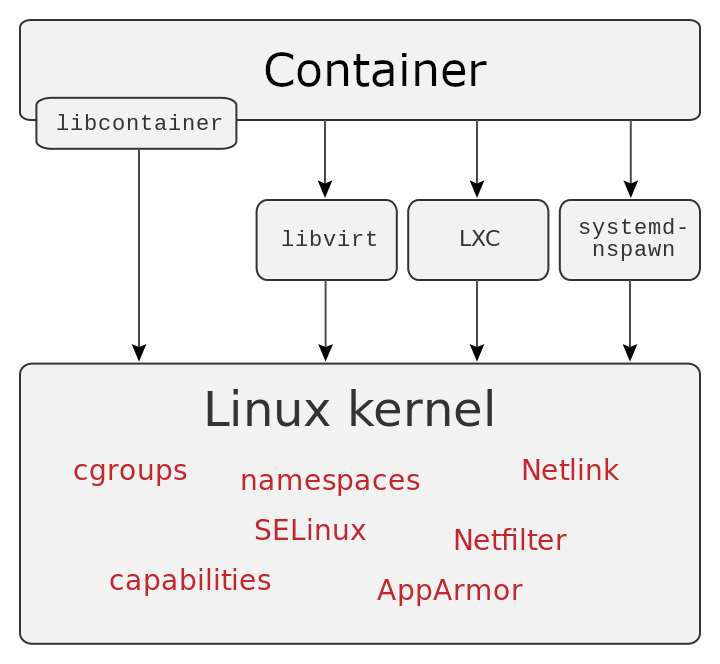
\includegraphics[width=0.7\textwidth]{LinuxKernelContainer.png}
	\end{center}
	\caption[Schnitstelle vom Container zum Kernel]{Schnitstelle vom Container zum Kernel \footnotemark}
	\label{fig:Schnittstelle}
\end{figure}
\quellefoot{4}{https://de.wikipedia.org/wiki/Docker_(Software)\#/media/File:Docker-linux-interfaces.svg}

